% coucou

\section{Results}
 
\subsection{Pressurized Water Reactor}

\subsubsection{Output analyses}
Figure~(\ref{fig:PWR_MOX_FLM_Pu.pdf}) presents the plutonium fraction at BOC predicted by each FLM and the plutonium fraction at EOC deduced by each software. As all FLM are different, the BOC plutonium fractions differ from a software from another. The wider prediction is given by the CLASS code that predicts plutonium fraction from 4\% until more that 15\%. This range is a direct consequence of the plutonium sampling used for this work. 15\% is clearly unrealistic but some of the plutonium isotopic composition sampled are not eather by containing a low amount of fissile. That'is why the FLMs may reach such high values.   

\begin{figure}[h]
	\begin{center}
		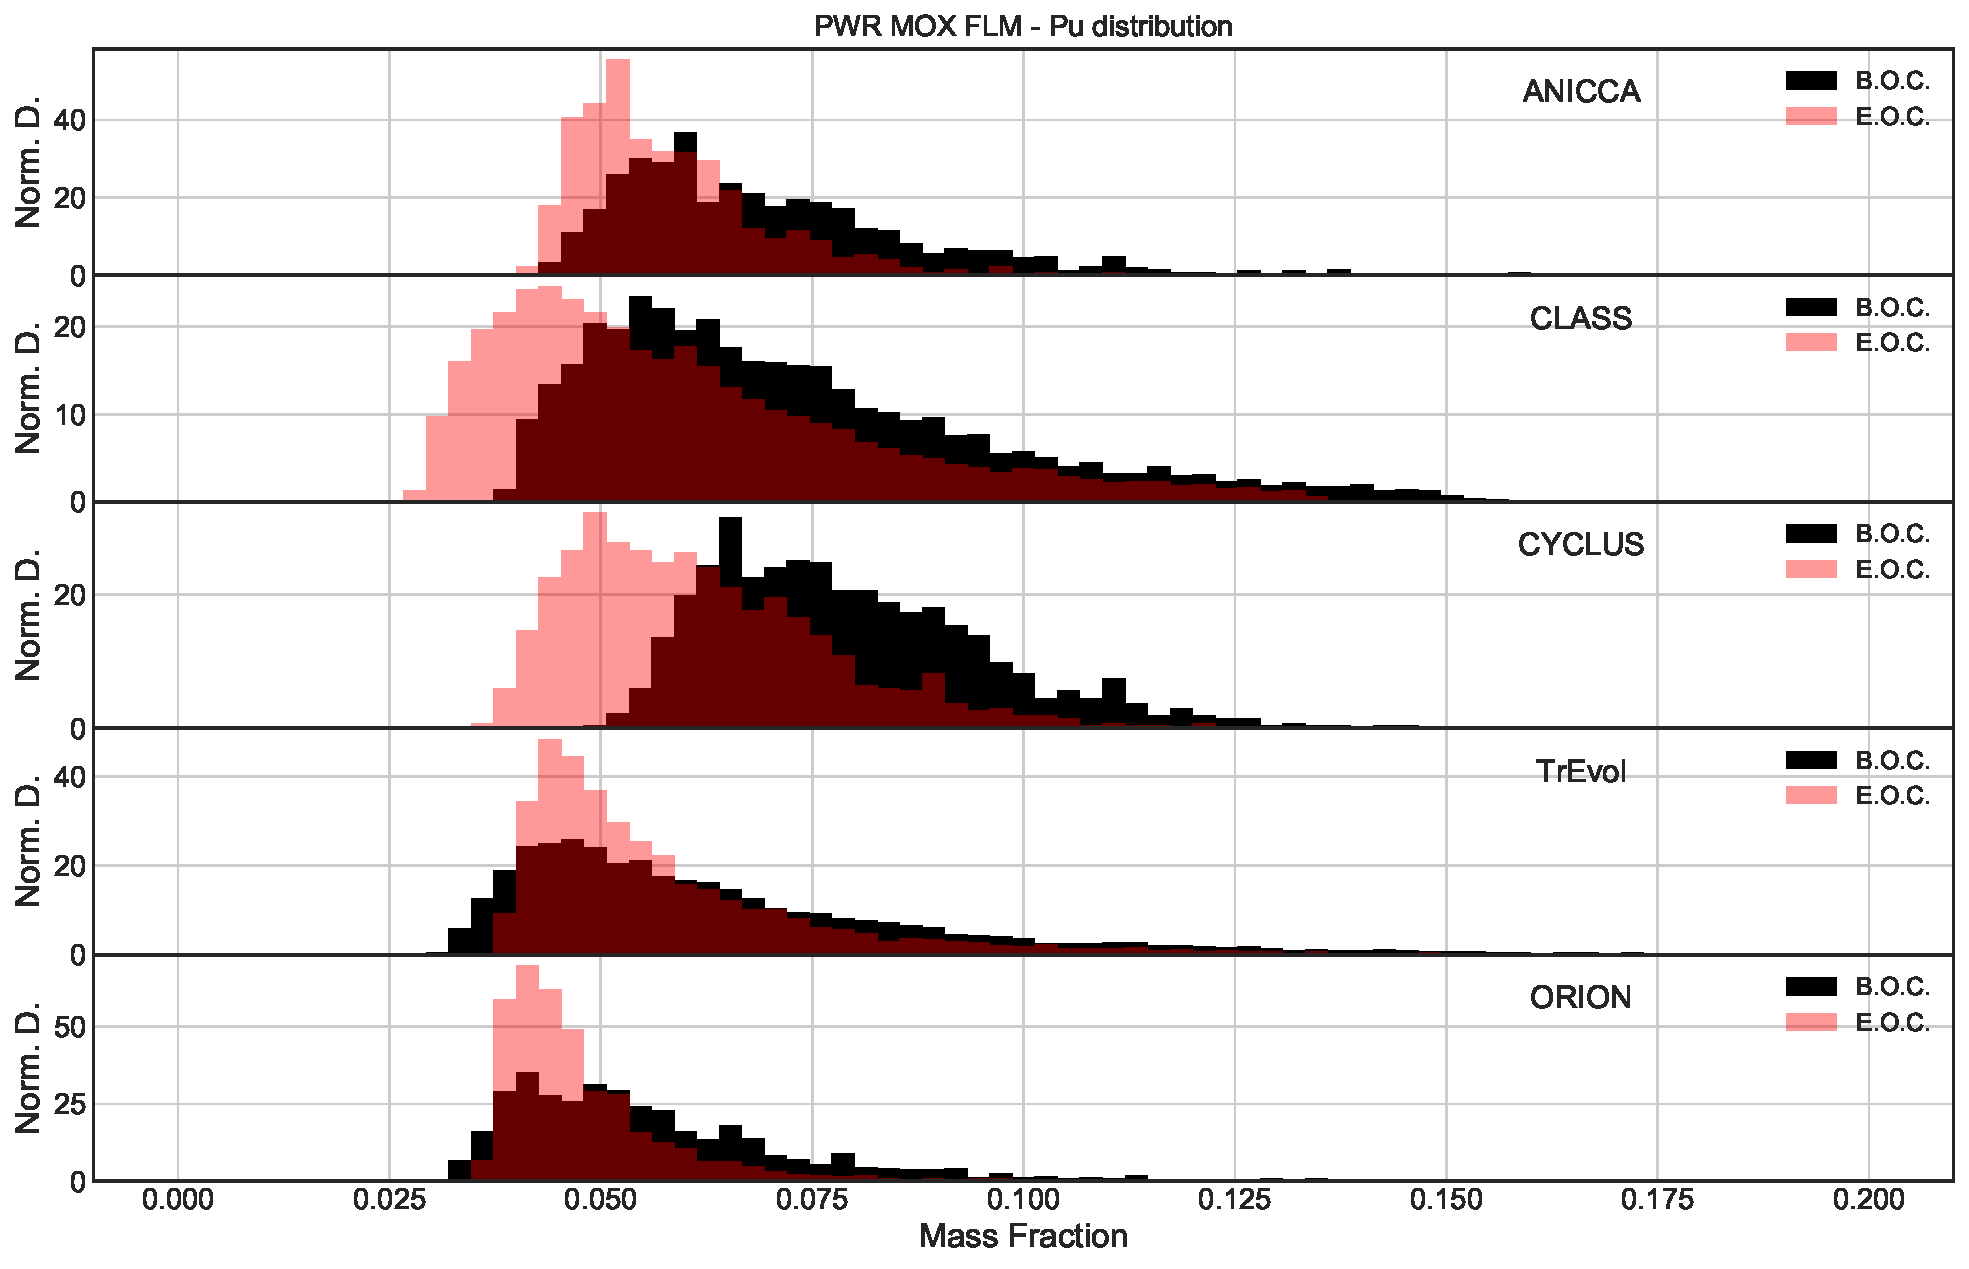
\includegraphics[width = 0.99\textwidth]{../../Feature_1/RAW_DATA/FIG/PWR_MOX_FLM_Pu.pdf}
		\caption{Code outputs for PWR scenario's calculations}
		\label{fig:PWR_MOX_FLM_Pu.pdf}
	\end{center}
\end{figure}

The EOC plutonium fraction is clearly shiffted to the lower values, proving that plutonium is consumed during irradiation like it should be in PWRs.   

\subsubsection{Estimator's calculation}

Figure~(\ref{fig:Est1_PWR}), figure~(\ref{fig:Est2_PWR}) and figure~(\ref{fig:Est3_PWR}) presents the calculation results for PWR of the different estimators defined in the previous section. 

\paragraph{Plutonium fraction at BOC}
Estimator 1 aims to quantify biais introduced by the use of a FF model on the plutonium enrichment for fresh MOX fuel. It measures the amount of plutonium taken from UOX spent fuel for MOX fuel fabrication. As it can be seen, 

\begin{figure}[h]
	\begin{center}
		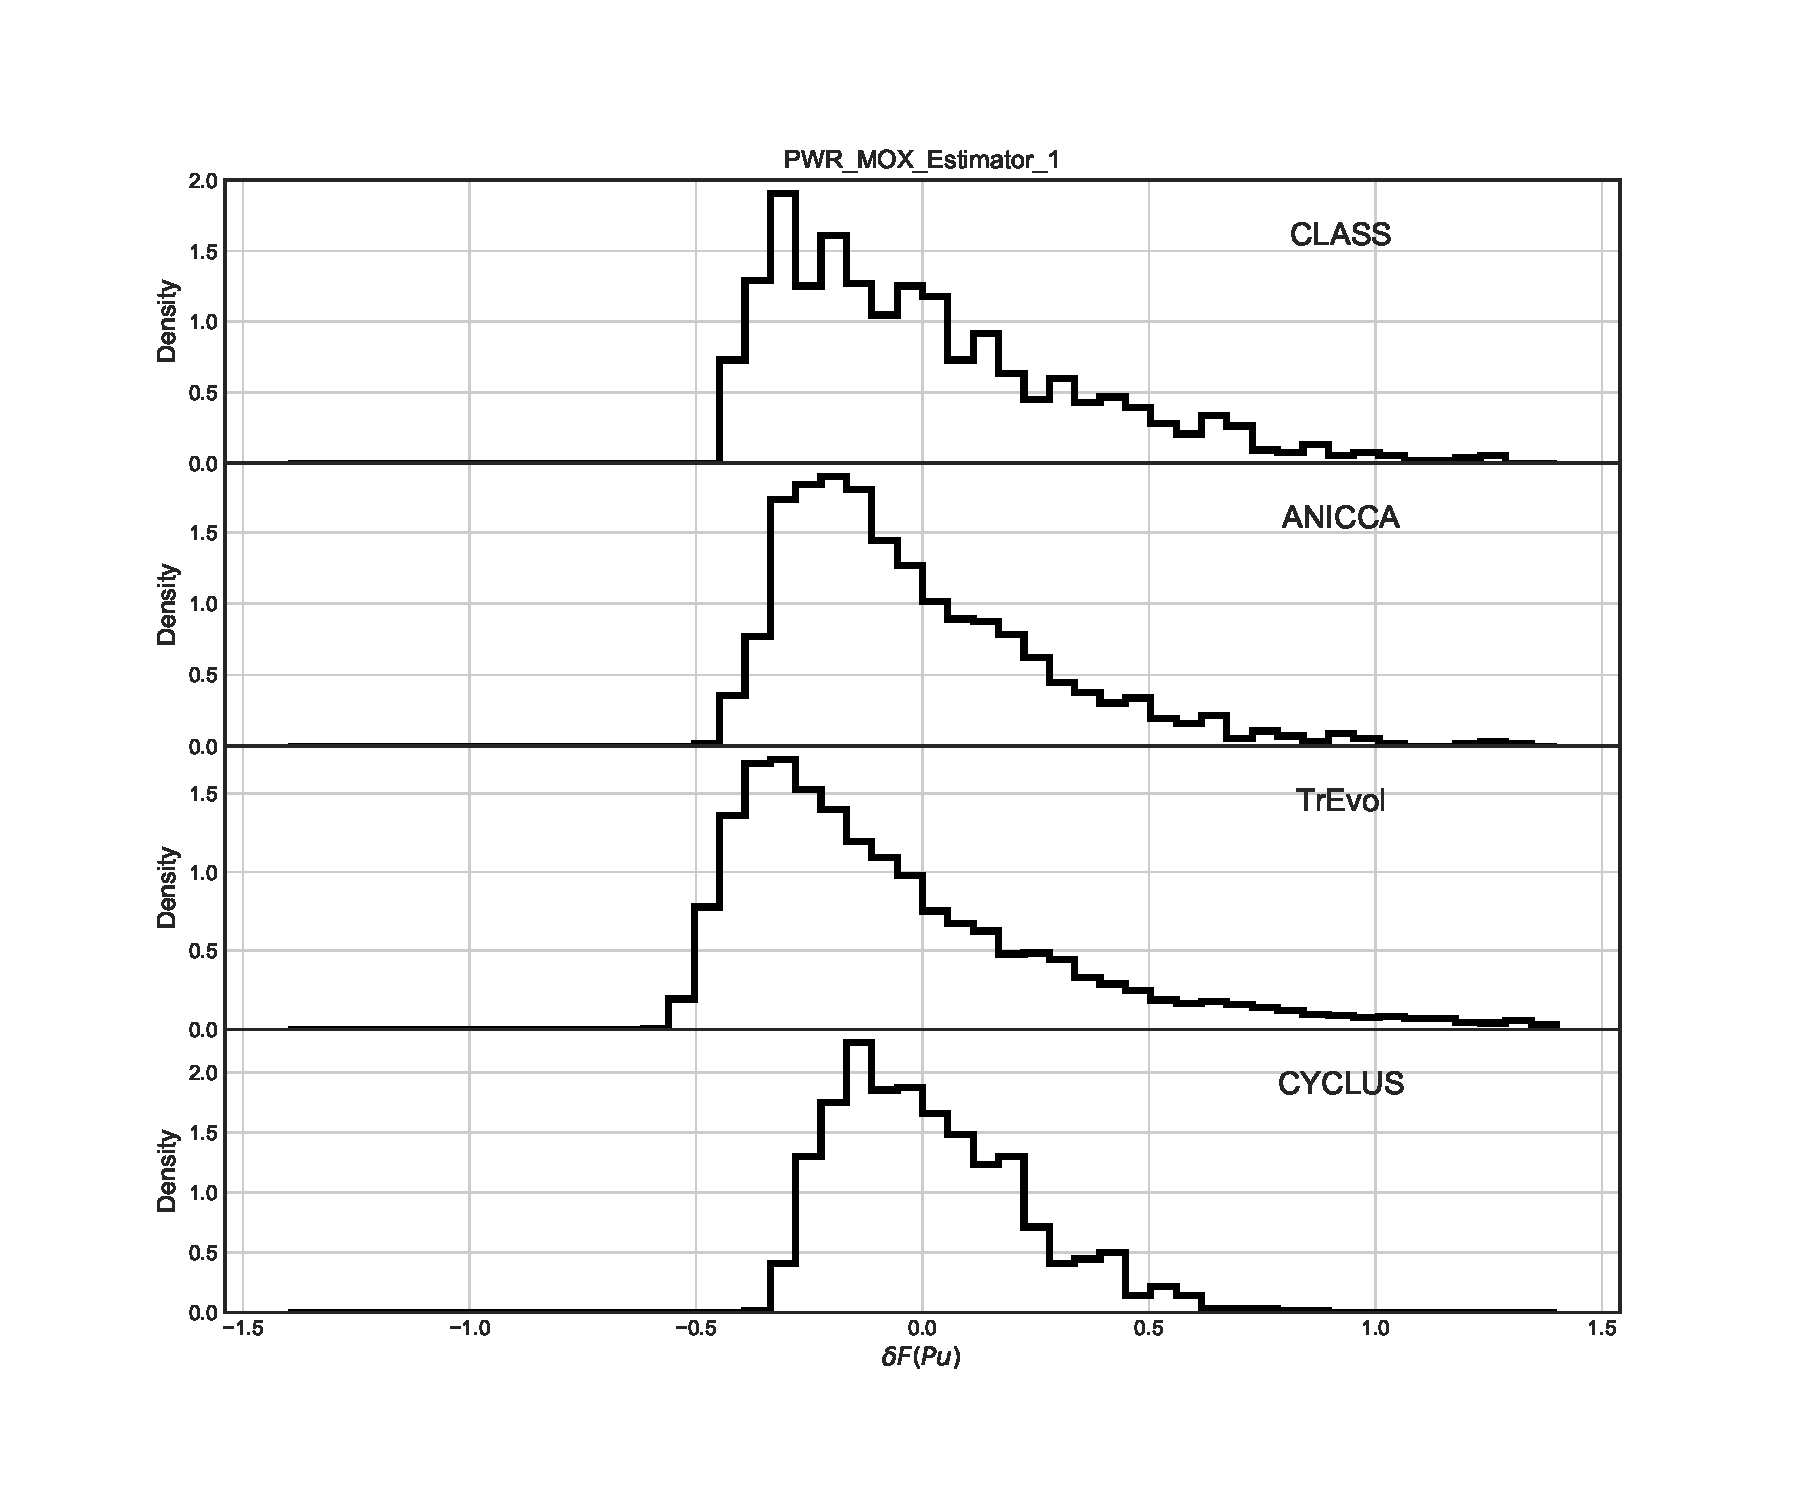
\includegraphics[width = 0.99\textwidth]{../../Feature_1/RAW_DATA/FIG/PWR_MOX_Estimator_1.pdf}
		\caption{Estimator 1 for PWR calculated with ANICCA, CLASS, CYCLUS and TrEVOL}
		\label{fig:Est1_PWR}
	\end{center}
\end{figure}

\paragraph{Ratio between plutonium consumption and plutonium at BOC}
\begin{figure}[h]
	\begin{center}
		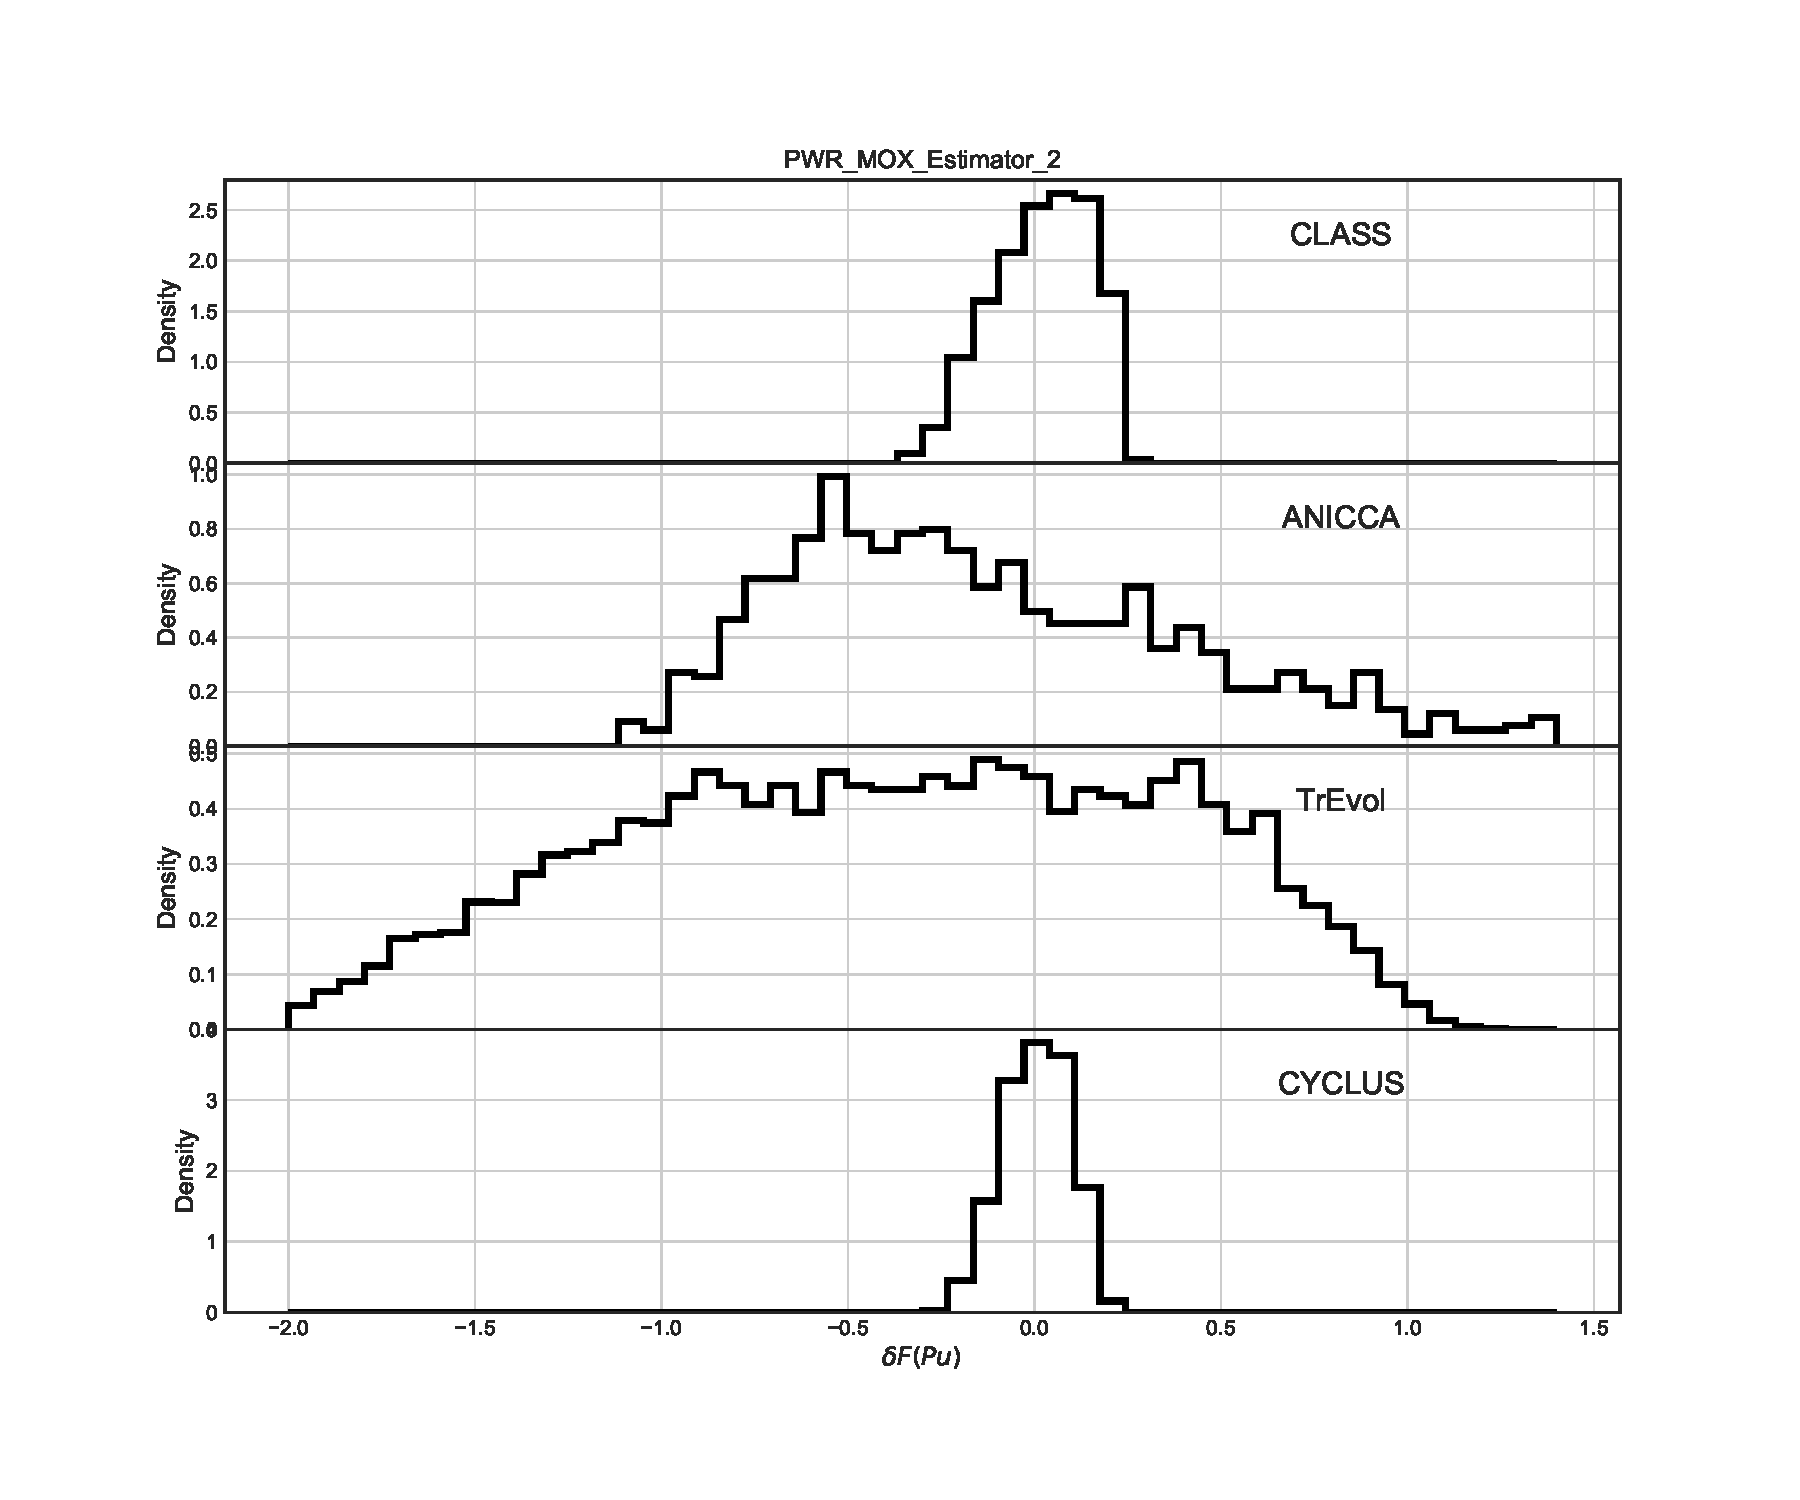
\includegraphics[width = 0.99\textwidth]{../../Feature_1/RAW_DATA/FIG/PWR_MOX_Estimator_2.pdf}
		\caption{Estimator 2 for PWR calculated with CLASS, CYCLUS and TrEVOL}
		\label{fig:Est2_PWR}
	\end{center}
\end{figure}


\paragraph{Plutonium consumption rate}
\begin{figure}[h]
	\begin{center}
		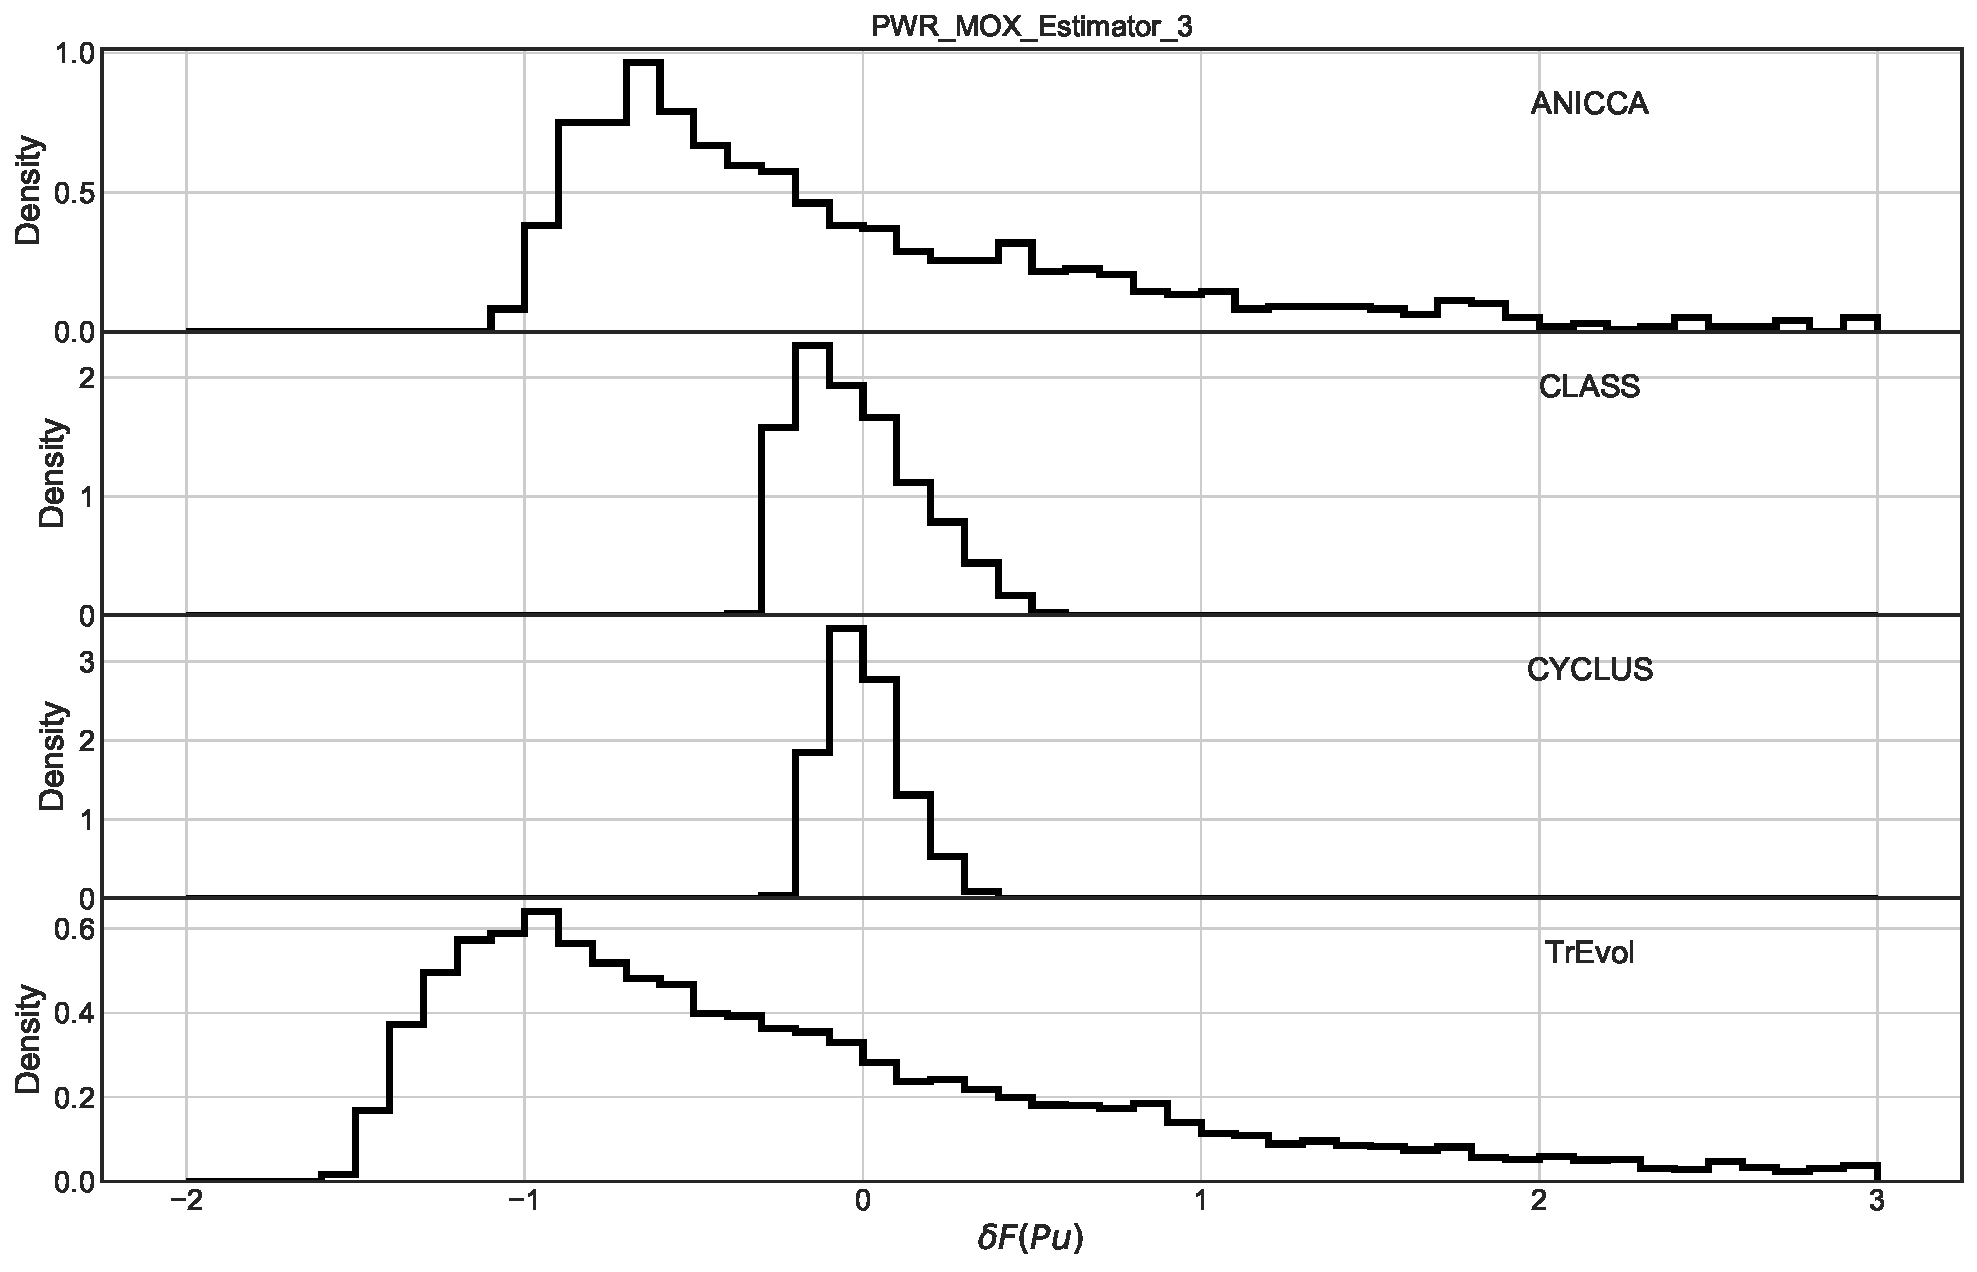
\includegraphics[width = 0.99\textwidth]{../../Feature_1/RAW_DATA/FIG/PWR_MOX_Estimator_3.pdf}
		\caption{Estimator 3 for PWR calculated with CLASS, CYCLUS and TrEVOL}
		\label{fig:Est3_PWR}
	\end{center}
\end{figure}

\subsection{Fast Sodium cooled Reactor}

Figure~\ref{fig:Est1_SFR} represents the estimator 1 calculated for Sodium Cooled Fast Reactors calculated with JOSETTE, TrEVOL and CLASS. Like for PWR, it shows the relative difference of plutonium enrichment with the use of a FLM in regards to a FF. Standard deviations of the difference distribution is given in Table~\ref{table:Est1Dev_SFR} for the different codes. 
All codes are in agreement even if CLASS slightly underestimate the FF impact on the plutonium needed for a SFR. The typical biais produced by the use of a FF is smaller than 25\% and is much lower than for PWR.  

\begin{figure}[h]
	\begin{center}
		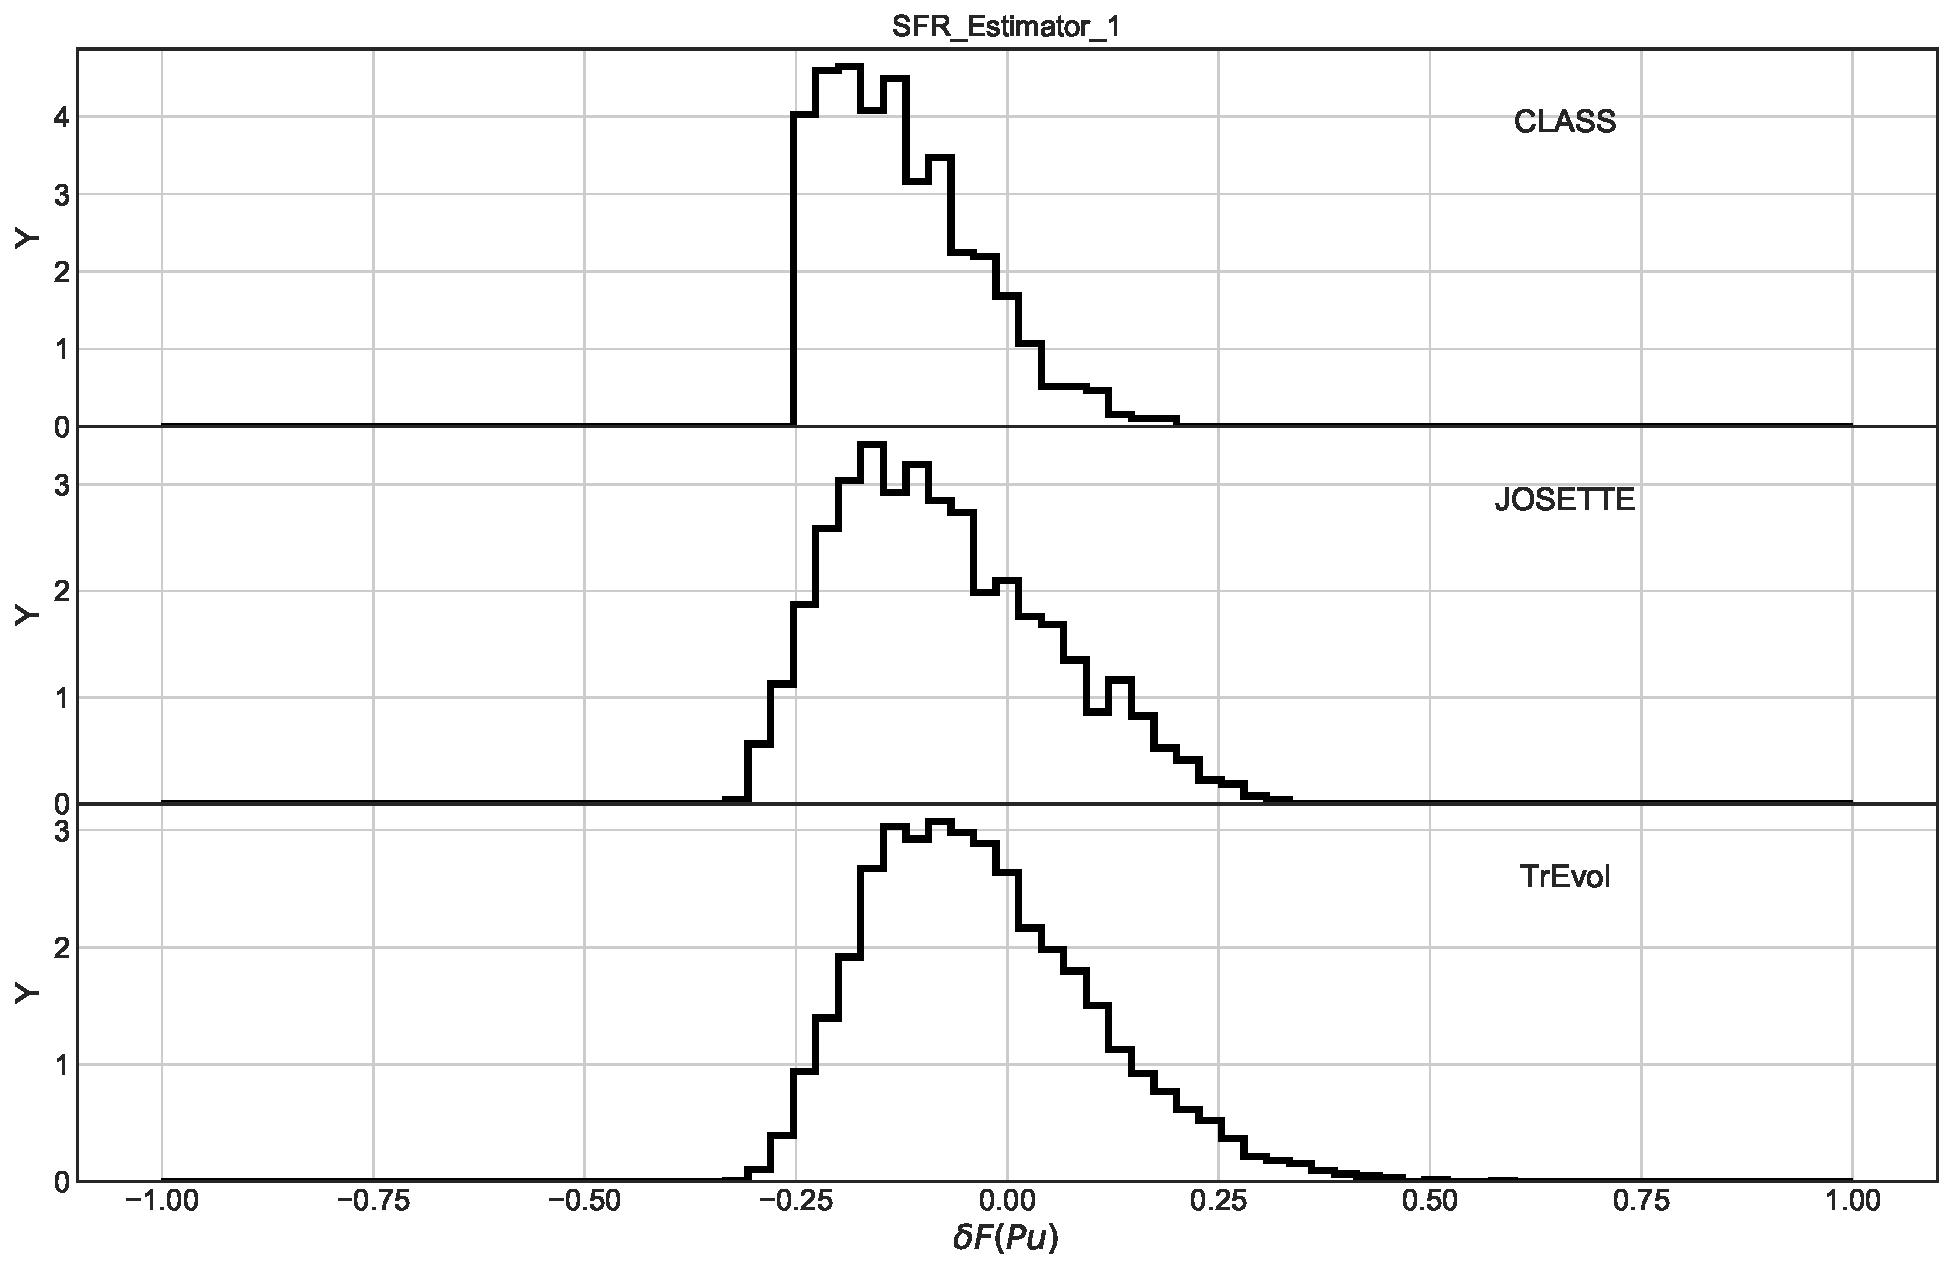
\includegraphics[width = 0.99\textwidth]{../../Feature_1/RAW_DATA/FIG/SFR_Estimator_1.pdf}
		\caption{Estimator 1 for SFR calculated with JOSETTE, TrEVOL, and CLASS}
		\label{fig:Est1_SFR}
	\end{center}
\end{figure}

\begin{table}[h]
	\begin{center}
		\begin{tabular}{|c||c||c|}
			\hline 
				JOSETTE & TrEVOL & CLASS \\
			\hline
				XX & YY & ZZ \\
		\end{tabular}
	\end{center}
	\label{table:Est1Dev_SFR}
\end{table}

\begin{figure}[h]
	\begin{center}
		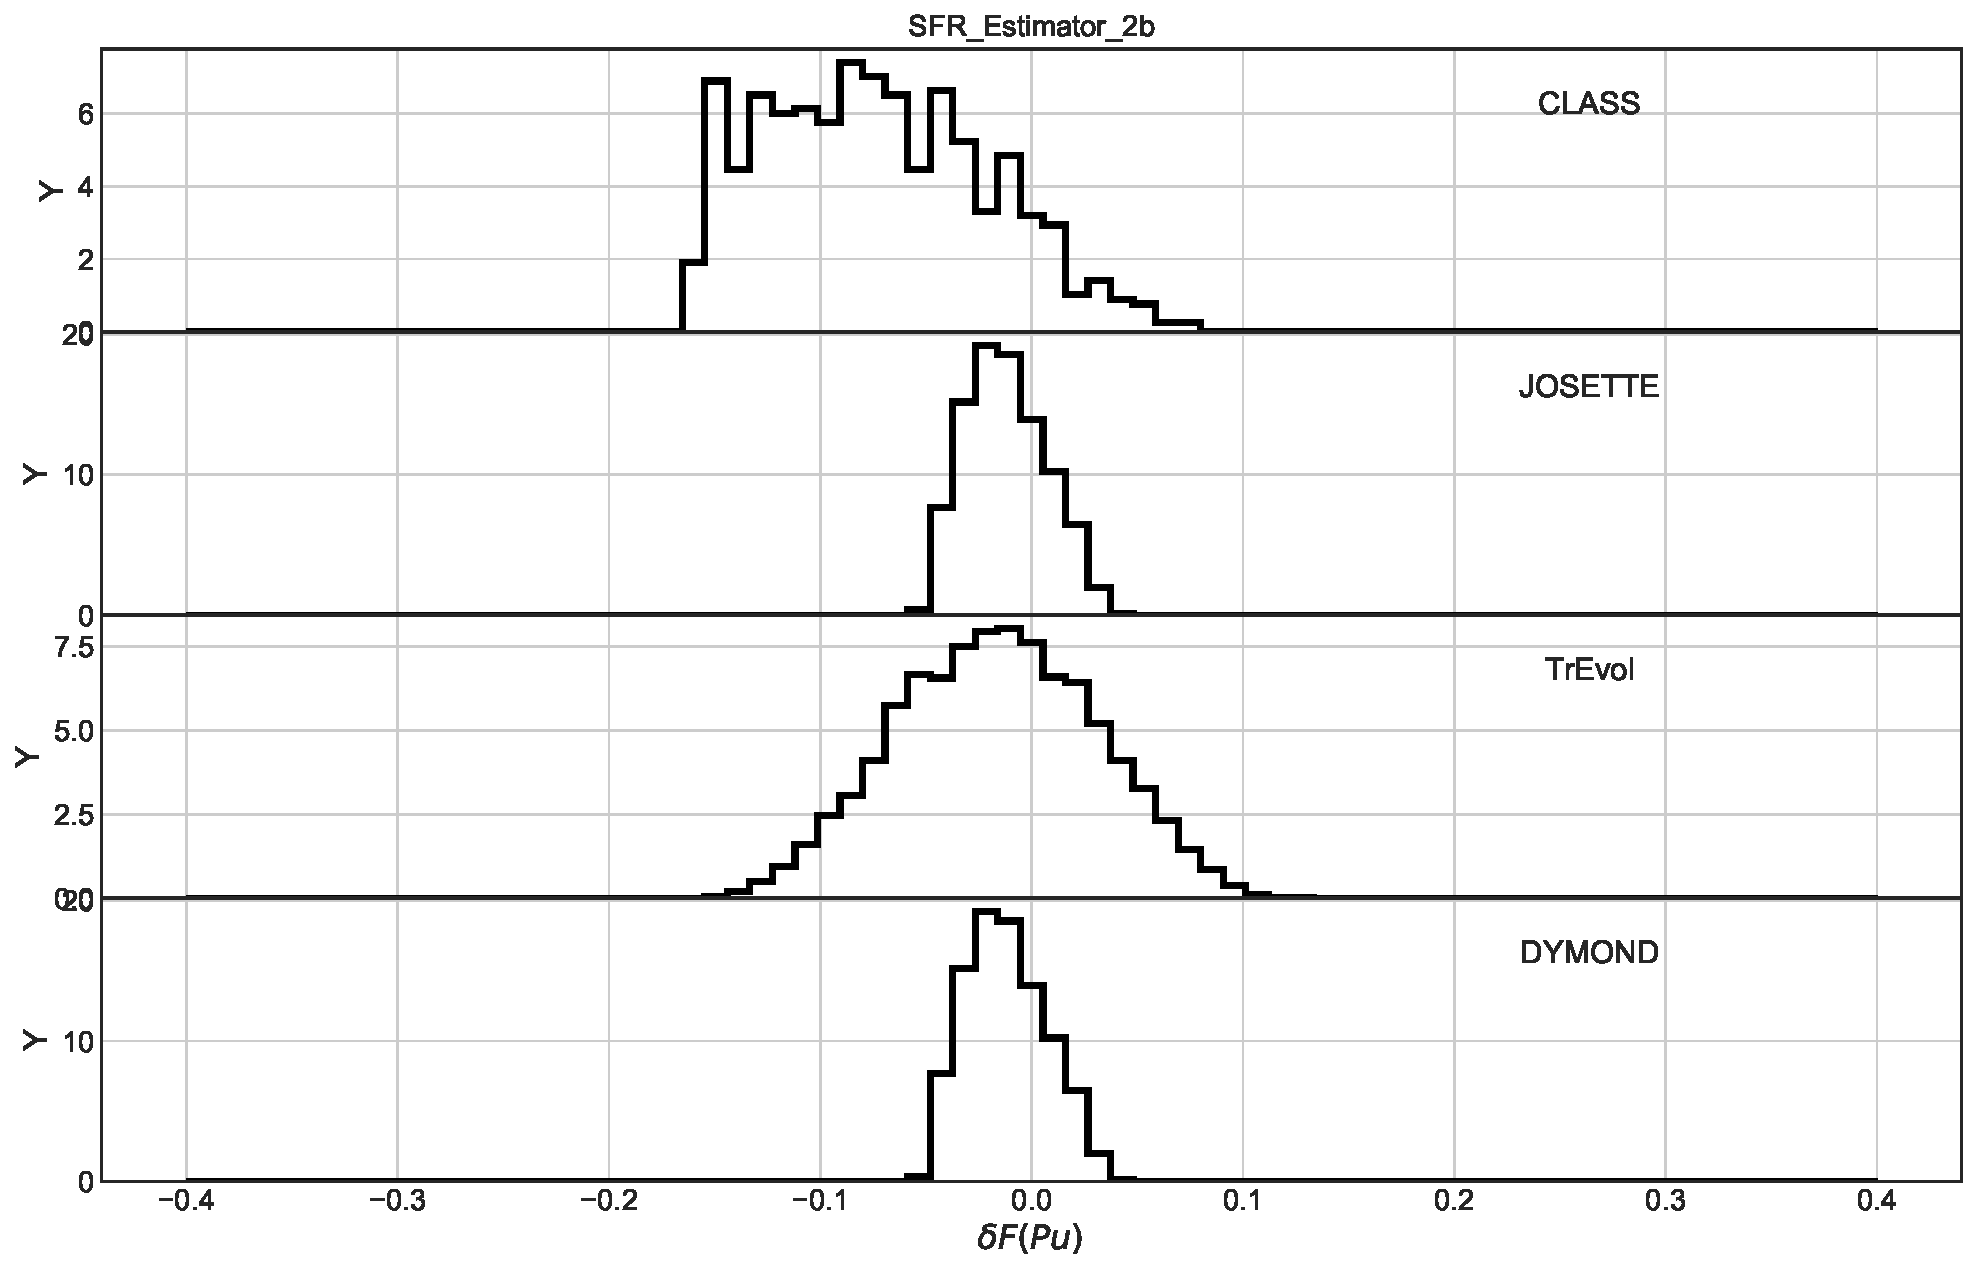
\includegraphics[width = 0.99\textwidth]{../../Feature_1/RAW_DATA/FIG/SFR_Estimator_2b.pdf}
		\caption{Estimator 2.b for SFR calculated with JOSETTE, TrEVOL, and CLASS}
		\label{fig:Est2_SFR}
	\end{center}
\end{figure}
